Not everything is rosy out there. Quoting @bulwarkonline@newsie.social:
\url{https://newsie.social/@bulwarkonline/110019522841620525} \#retoot

\begin{figure}
\centering
\pandocbounded{
\includegraphics[keepaspectratio]{\%7B\%7Bsite.url\%7D\%7D/img/regime-talk.jpg}}
\caption{Post by The Bulwark. ``\,``\,`Regime' rhetoric draws on three
main currents of formerly dissident right-wing thought: the Claremont
Institute's turn against America, the inverted Marxism of
paleoconservatives, and the techno-authoritarianism of Peter Thiel.''
ICYMI @Joshua\_A\_Tait: thebulwark.com/the-problem-wit\ldots'' Posted on
Mar 13, 2023 at 23:31}
\end{figure}

The referenced post can be found at
\url{https://www.thebulwark.com/the-problem-with-right-wing-regime-talk/}.

It looks like we're not out of the woods yet with the incipient banking
crisis here in the USA. Even though the Financial Stability Oversight
Council made a statement on Monday they don't have control over events.
Quoting @Techmeme@techhub.social:
\url{https://techhub.social/@Techmeme/110019462416367870} \#retoot

\begin{figure}
\centering
\pandocbounded{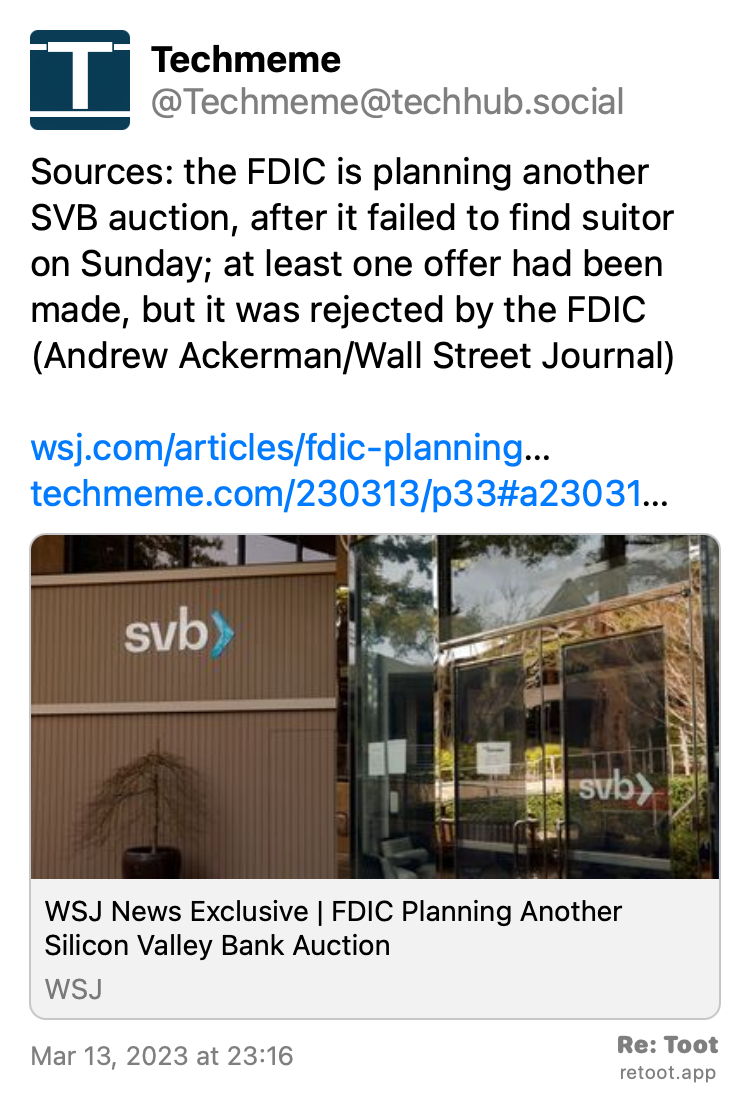
\includegraphics[keepaspectratio]{\%7B\%7Bsite.url\%7D\%7D/img/spook-markets.jpg}}
\caption{Post by Techmeme. ``Sources: the FDIC is planning another SVB
auction, after it failed to find suitor on Sunday; at least one offer
had been made, but it was rejected by the FDIC (Andrew Ackerman/Wall
Street Journal) wsj.com/articles/fdic-planning\ldots{}
techmeme.com/230313/p33\#a23031\ldots{}'' Posted on Mar 13, 2023 at
23:16}
\end{figure}

The original post on Techmeme is at
\url{http://www.techmeme.com/230313/p33\#a230313p33}. I think that
\emph{this} will spook people and create instability again. We'll see
what happens. First Commonwealth, PNC, Fifth Third, Huntington, and
other regional banks serving my immediate area got \emph{pounded} quite
hard in stock trading Monday.

Steve Herman at the Voice of America brought news over the weekend that
we're in bad shape as to news-seeking behavior by the public. Facebook
is a farrago of lies and deceit. Where do most Americans go online to
get their news? Facebook! Quoting @w7voa@journa.host:
\url{https://journa.host/@w7voa/110012130279790977} \#retoot

\begin{figure}
\centering
\pandocbounded{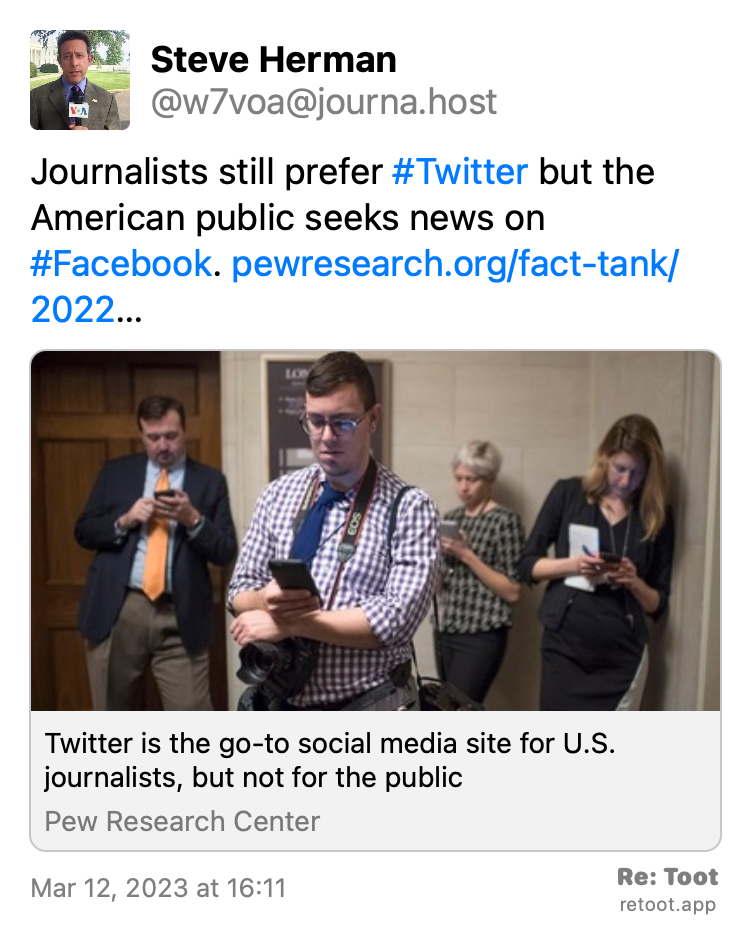
\includegraphics[keepaspectratio]{\%7B\%7Bsite.url\%7D\%7D/img/the-fb-problem.jpg}}
\caption{Post by Steve Herman. ``Journalists still prefer \#Twitter but
the American public seeks news on \#Facebook.
pewresearch.org/fact-tank/2022\ldots{}'' Posted on Mar 12, 2023 at
16:11}
\end{figure}

The linked report can be seen at
\url{https://www.pewresearch.org/fact-tank/2022/06/27/twitter-is-the-go-to-social-media-site-for-u-s-journalists-but-not-for-the-public/}.

I agree with Alan Pope that the news is not good right now.
